\chapter{Machine Translation \cite{dnn-1}} \label{chapter: Machine Translation}

\begin{enumerate}
    \item model is presented with a sentence in one language and must predict the corresponding sentence in another. 
    
    \item Note that here the sentences may be of different lengths, and that corresponding words in the two sentences may not occur in the same order, owing to differences in the two language’s grammatical structure.

    \item Many problems have this flavor of mapping between two such “unaligned” sequences.\\
    \textbf{Examples} include mapping from dialog prompts to replies or from questions to answers. \\
    Broadly, such problems are called \textbf{sequence-to-sequence (seq2seq) problems}
\end{enumerate}

\vspace{0.5cm}
\noindent
\textbf{Preprocessing}:
\begin{enumerate}
    \item \textbf{Tokenization}
    \begin{enumerate}
        \item We append the special “<eos>” token to the end of every sequence to indicate the \textbf{end of the sequence}.
        
        \item When a model is predicting by generating a sequence token after token, the generation of the “<eos>” token can suggest that the output sequence is complete. 

    \end{enumerate}

\end{enumerate}


\section{Encoder–Decoder Architecture \cite{dnn-1}} \label{Encoder–Decoder Architecture}

\begin{figure}[H]
    \centering
    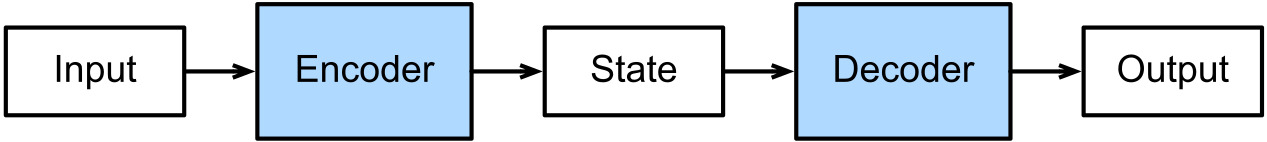
\includegraphics[width=\linewidth, height=1cm, keepaspectratio]{Pictures/Recurrent-Neural-Networks/encoder-decoder.jpg}
\end{figure}

\begin{customTableWrapper}{1.5}
\begin{longtable}{l p{8cm}}
    \hline
    \customTableHeaderColor
    \multicolumn{2}{c}{Encoder} \\ \hline
    
    $T$ & number of time steps/ length of input sequence \\

    $t$ & time step \\

    $x_1, \ldots, x_T$ & input sequence \\

    $x_t$ & token at $t^{th}$ time step/ $t^{th}$ token \\

    \hline

    $\mathbf{x}_t$ & transformed input feature vector \\

    \hline
    
    $\mathbf{h} _{t-1}$ & hidden state from the previous time step \\

    $f$ & transformation function of the RNN’s recurrent layer \\

    $\mathbf{h}_t$ & current hidden state \\

    \hline

    $q$ & customized function to transform the hidden states at all time steps into a context variable \\
    
    $\mathbf{c}$ &  fixed-shape context variable \\

    \hline
    \customTableHeaderColor
    \multicolumn{2}{c}{Decoder} \\ \hline

    $T^\prime$ & total time steps \\

    $t^\prime$ & time step \\

    $y_1, y_2, \ldots, y_{T^\prime}$ & target output sequence \\

    $\mathbf{s}_{t^\prime-1}$ & hidden RNN state from the previous time step \\

    $g$ & transformation function  \\

    $\mathbf{s}_{t^\prime}$ & hidden state at the current time step \\
\end{longtable}
\end{customTableWrapper}

\begin{enumerate}
    \item The standard approach to handling inputs and outputs are of varying lengths that are unaligned data is to design an encoder–decoder architecture consists of two major components: 
    \begin{enumerate}
        \item an encoder that takes a variable-length sequence as input
        
        \item a decoder that acts as a conditional language model, taking in the encoded input and the leftwards context of the target sequence and predicting the subsequent token in the target sequence.
    \end{enumerate}

    \item the entire input was compressed by the encoder into a single fixed-length vector to be fed into the decoder.     
\end{enumerate}




\subsection{Encoder \cite{dnn-1}} \label{rnn: Encoder}

\begin{enumerate}
    \item encoder transforms an input sequence of variable length into a fixed-shape context variable $\mathbf{c}$

    \item At time step $t$, the RNN transforms the input feature vector $\mathbf{x}_t$ for $x_t$ and the hidden state $\mathbf{h}_{t-1}$ from the previous time step into the current hidden state $\mathbf{h}_{t}$. 
    
    \item We can use a function $f$ to express the transformation of the RNN’s recurrent layer:
    $
        \hfill
        \mathbf{h}_t = f(\mathbf{x}_t, \mathbf{h}_{t-1})
        \hfill
    $

    \item $\mathbf{c} =  q(\mathbf{h}_1, \ldots, \mathbf{h}_T)$

    \item the context variable is just the hidden state $\mathbf{h}_T$ corresponding to the encoder RNN’s representation after processing the final token of the input sequence.

    \item we use an \textbf{embedding layer} to obtain the feature vector for each token in the input sequence.\\
    The weight of an embedding layer is a matrix, where the number of rows corresponds to the size of the input vocabulary (\verb|vocab_size|) and number of columns corresponds to the feature vector’s dimension (\verb|embed_size|).\\
    For any input token index $i$, the embedding layer fetches the $i^{th}$ row (starting from 0) of the weight matrix to return its feature vector.\\
    Here we implement the encoder with a multilayer GRU.
\end{enumerate}


\subsubsection{Teacher Forcing \cite{dnn-1}} \label{Teacher Forcing}

\begin{enumerate}
    \item While running the encoder on the input sequence is relatively straightforward, handling the input and output of the decoder requires more care. 
    
    \item The most common approach is sometimes called teacher forcing. 
    
    \item Here, the original target sequence (token labels) is fed into the decoder as input. 
    
    \item More concretely, the special beginning-of-sequence token and the original target sequence, excluding the final token, are concatenated as input to the decoder, while the decoder output (labels for training) is the original target sequence, shifted by one token:\\
    “<bos>”, “Ils”, “regardent”, “.” $\rightarrow$ “Ils”, “regardent”, “.”, “<eos>”.

    \item An alternative approach is to feed the predicted token from the previous time step as the current input to the decoder.

\end{enumerate}





\subsection{Decoder \cite{dnn-1}} \label{rnn: Decoder}

\begin{enumerate}
    \item the decoder assigns a predicted probability to each possible token occurring at step $y_{t^\prime+1}$ conditioned upon the previous tokens in the target $y_1, \ldots, y_{t^\prime}$ and the context variable $\mathbf{c}$, i.e., $P(y_{t^\prime+1} \mid y_1, \ldots, y_{t^\prime}, \mathbf{c})$

    \item To predict the subsequent token $t^\prime+1$ in the target sequence, the RNN decoder takes the previous step’s target token $y_{t^\prime}$, the hidden RNN state from the previous time step $\mathbf{s}_{t^\prime-1}$, and the context variable $\mathbf{c}$ as its input, and transforms them into the hidden state $\mathbf{s}_{t^\prime}$ at the current time step.\\
    We can use a function $g$ to express the transformation of the decoder’s hidden layer:
    $
        \hfill
        \mathbf{s}_{t^\prime} = g(y_{t^\prime-1}, \mathbf{c}, \mathbf{s}_{t^\prime-1})
        \hfill
    $

    \item After obtaining the hidden state of the decoder, we can use an output layer and the softmax operation to compute the predictive distribution $p(y_{t^{\prime}+1} \mid y_1, \ldots, y_{t^\prime}, \mathbf{c})$ over the subsequent output token ${t^\prime+1}$

    
\end{enumerate}









\section{Sequence-to-Sequence Learning for Machine Translation \cite{dnn-1}}

\begin{figure}[H]
    \centering
    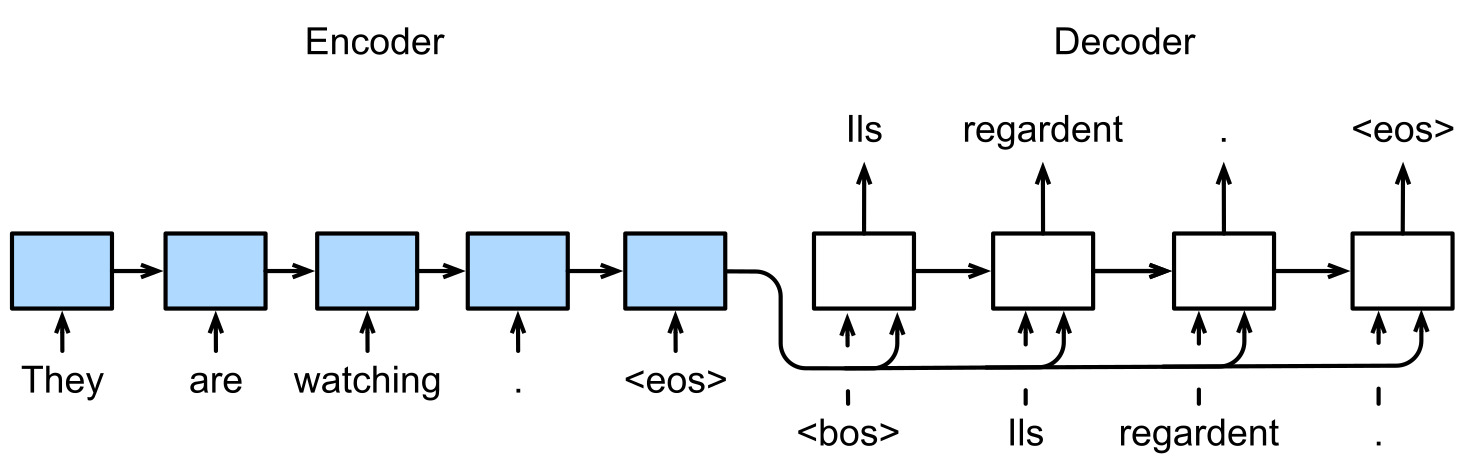
\includegraphics[width=\linewidth, height=2.5cm, keepaspectratio]{Pictures/Recurrent-Neural-Networks/seq2seq-nmt.jpg}
\end{figure}


\begin{enumerate}[itemsep=0.15cm]
    \item the encoder RNN will take a variable-length sequence as input and transform it into a fixed-shape hidden state

    \item to generate the output sequence, one token at a time, the decoder model, consisting of a separate RNN, will predict each successive target token given both the input sequence and the preceding tokens in the output. 
    
    \item During training, the decoder will typically be conditioned upon the preceding tokens in the official “ground truth” label. However, at test time, we will want to condition each output of the decoder on the tokens already predicted. 
    
    \item Note that if we ignore the encoder, the decoder in a sequence-to-sequence architecture behaves just like a normal language model.

    \item the special “<eos>” token marks the end of the sequence. 
    
    \item Our model can stop making predictions once this token is generated.\\
    At the initial time step of the RNN decoder, there are two special design decisions to be aware of: 
    \begin{enumerate}
        \item we begin every input with a special beginning-of-sequence “<bos>” token. 
    
        \item we may feed the final hidden state of the encoder into the decoder at every single decoding time step. 
    \end{enumerate}
    
    \item In some other designs, the final hidden state of the RNN encoder is used to initiate the hidden state of the decoder only at the first decoding step.


\end{enumerate}


\subsection{Evaluation of Predicted Sequences}

SEE: \fullref{Bilingual Evaluation Understudy (BLEU)}


\section{Searching}

\begin{customTableWrapper}{1.5}
\begin{longtable}{l p{8cm}}
    $T^\prime$ & maximum number of tokens of an output sequence \\
    
    $t^\prime$ & time step \\

    $y_{t^\prime}$ & token \\

    $\mathcal{Y}$ & output vocabulary (including the special end-of-sequence token “\verb|<eos>|”) \\
\end{longtable}
\end{customTableWrapper}


\subsection{Greedy Search \cite{dnn-1}} \label{nmt: Greedy Search}

\begin{enumerate}[itemsep=0.15cm]
    \item Our goal is to search for an ideal output from all $\mathcal{O}(\left|\mathcal{Y}\right|^{T'})$ possible output sequences

    \item $y_{t'} = \operatorname*{argmax}_{y \in \mathcal{Y}} P(y \mid y_1, \ldots, y_{t'-1}, \mathbf{c})$

    \item Once our model outputs “\verb|<eos>|” (or we reach the maximum length $T^\prime$) the output sequence is completed

    \item if we put aside efficiency for a minute, it might seem more reasonable to search for the \textbf{most likely sequence}, not the sequence of (greedily selected) \textbf{most likely tokens}.\\
    It turns out that these two objects can be quite different.\\
    The most likely sequence is the one that maximizes the expression $\dprod_{t'=1}^{T'} P(y_{t'} \mid y_1, \ldots, y_{t'-1}, \mathbf{c})$

   \item computational cost of greedy search: $\mathcal{O}(\left|\mathcal{Y}\right|T')$\\
   miraculously cheap but far from optimal
\end{enumerate}

\subsection{Exhaustive Search \cite{dnn-1}} \label{nmt: Exhaustive Search}

\begin{enumerate}
    \item enumerate all the possible output sequences with their conditional probabilities, and then output the one that scores the highest predicted probability.

    \item prohibitive computational cost: $\mathcal{O}(\left|\mathcal{Y}\right|^{T'})$

\end{enumerate}


\subsection{Beam Search \cite{dnn-1}} \label{nmt: Beam Search}

\begin{figure}[H]
    \centering
    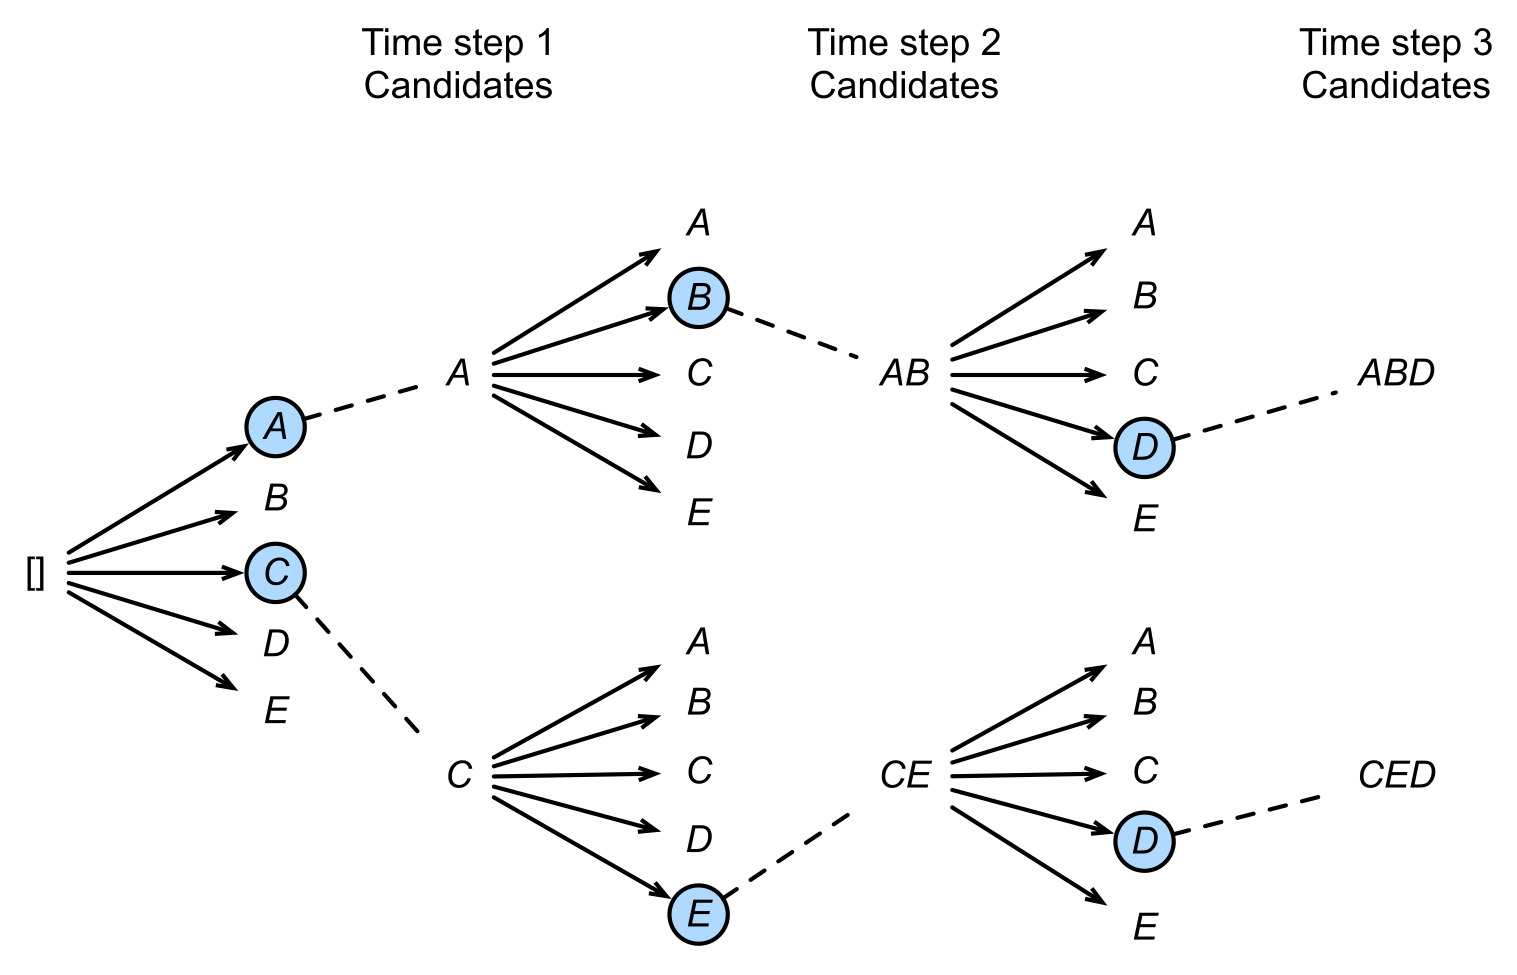
\includegraphics[width=\linewidth, height=5cm, keepaspectratio]{Pictures/Recurrent-Neural-Networks/nmt-beam-search.jpg}
\end{figure}

\begin{customTableWrapper}{1.5}
\begin{longtable}{l p{8cm}}
    $k$ & beam size \\

    $L$ & length of the final candidate sequence \\

    $\alpha$ & \\

\end{longtable}
\end{customTableWrapper}

\begin{enumerate}
    \item beam search striks a compromise between the efficiency of greedy search and the optimality of exhaustive search.

    \item The most straightforward version of beam search is characterized by a single hyperparameter, the beam size, $k$

    \item At time step 1, we select the $k$ tokens with the highest predicted probabilities.\\
    Each of them will be the first token of $k$ candidate output sequences, respectively.\\
    At each subsequent time step, based on the $k$ candidate output sequences at the previous time step, we continue to select $k$ candidate output sequences with the highest predicted probabilities from $k\left|\mathcal{Y}\right|$ possible choices.

    \item In the end, we obtain the set of final candidate output sequences based on these six sequences (e.g., discard portions including and after “\verb|<eos>|”). Then we choose the output sequence which maximizes the following score:
    
    \item[] $
        \hfill
        \frac{1}{L^\alpha} \log P(y_1, \ldots, y_{L}\mid \mathbf{c}) = \dfrac{1}{L^\alpha} \sum_{t'=1}^L \log P(y_{t'} \mid y_1, \ldots, y_{t'-1}, \mathbf{c})
        \hfill
    $
    
    \item $\alpha$ is usually set to $0.75$

    \item Since a longer sequence has more logarithmic terms in the summation, the term $L^\alpha$ in the denominator penalizes long sequences.

    \item computational cost of beam search: $\mathcal{O}(k\left|\mathcal{Y}\right|T')$

    \item Greedy search can be treated as a special case of beam search arising when the beam size is set to 1.

\end{enumerate}





























